\documentclass{beamer}
\usetheme{Boadilla}
\usepackage{color} 
\usepackage{graphicx}
\usepackage[latin1]{inputenc}
\usepackage[T1]{fontenc}
\usepackage[francais]{babel}
\usepackage{dsfont}
\usepackage{graphicx}
            

\title{\'Etude du syst\`eme d'OTP \og{}HOTP\fg{}}

\author{G. Ferry, M. Michotte, B. Zigh} 
\institute{Universit\'e de Rouen}
\date{3 D\'ecembre 2013} 

\AtBeginSection[] 
{ 
\begin{frame}  
\frametitle{Plan} 
\tableofcontents[currentsection,hideothersubsections]
\end{frame}
} 
\AtBeginSubsection[] 
{ 
\begin{frame}  
\frametitle{Plan} 
\tableofcontents[currentsubsection,hideothersubsections,subsectionstyle=show/shaded]
\end{frame}
} 

\begin{document}

\begin{frame} 
\titlepage
\end{frame}

\section{Pr\'erequis}

\begin{frame} 
\frametitle{En Bref}

\begin{block}{HOTP...}
\begin{itemize}
\item ... est bas\'e sur OTP (RFC 2289).
\pause \item ...repose sur l'utilisation du m\'ecanisme d'authentification de message HMAC (RFC 2104).
\end{itemize}  
\end{block}

\end{frame}

\begin{frame} 
\frametitle{En Bref}

\begin{block}{HMAC...}
\begin{itemize}
\item ...sert \`a v\'erifier si un message n'a pas \'et\'e alt\'er\'e
et \`a authentifier l'exp\'editeur
\pause\item ...se base sur l'utilisation d'une fonction de hachage et d'un secret partag\'e.
\end{itemize}  
\end{block}

\pause
\begin{exampleblock}{Calcul}
$HMAC_K(M) = h(K \oplus opad || h(K \oplus ipad || M))$ 
\end{exampleblock}

\end{frame}

\begin{frame}
\frametitle{Principe}
\begin{itemize}
\item On envoie le HMAC du message sur un canal s\'ecuris\'e diff\'erent de celui utilis\'e pour la transmission.
\pause
\item Le destinataire,  v\'erifie l'authenticit\'e du message en calculant le code HMAC.
\end{itemize}


\end{frame}

\section{G\'en\'eralit\'es}

\begin{frame}
\frametitle{Les OTP}

\begin{itemize}
 \item N\'ecessitent d'\^etre attach\'es sur un syst\`eme classique de login/pass
 \pause\item Peuvent \^etre synchrones.
 \pause\item Peuvent \^etre asynchrones.
\end{itemize}
\end{frame}

\begin{frame}
\frametitle{HOTP est synchrone}
\begin{itemize}
 \item L'utilisateur demande \`a son token\footnote{Le token est un \'el\'ement mat\'eriel ou logiciel dont la seule fonction est de g\'en\'erer des mots de passe jetables.} de 
 g\'en\'erer un mot de passe jetable.
\pause \item Le token g\'en\`ere le mot de passe en calculant $HMAC_K(C)$, et incr\'emente le compteur.
\pause \item L'utilisateur r\'ecup\`ere le mot de passe jetable fourni par le token et le passe au serveur.
\pause \item Le serveur calcule $HMAC_K(C)$, et incr\'emente le compteur.
\pause \item Si la valeur calcul\'ee par le serveur coincide avec la valeur envoy\'ee par l'utilisateur, ce dernier est authentifi\'e. Dans le cas contraire, il est rejet\'e
\end{itemize}
\end{frame}

\begin{frame}
\frametitle{HOTP est un OTP}
On \'evite donc les attaques \og{}par rejeu\fg{}
\end{frame}

\section{Approfondissement}
\subsection{G\'en\'eration et partage d'un secret}
\begin{frame}
\frametitle{G\'en\'eration et partage d'un secret}
\og{}HOTP\fg{} propose pour la g\'en\'eration des secrets deux m\'ethodes : une m\'ethode d\'eterministe et une m\'ethode al\'eatoire. 
\end{frame}

 \subsubsection{M\'ethode d\'eterministe}
\begin{frame}
\frametitle{M\'ethode d\'eterministe 1/2}
\begin{block}{Description}
\begin{itemize}
\item Une clef maitresse, not\'ee $K_M$.
\pause\item Stock\'ee dans une zone s\'ecuris\'ee.
\pause\item $K_i$, personnelle pour chaque client (partag\'ee avec le serveur).
\pause\item Calcul\'ee \`a partir de la clef $K_M$ et d'une information, $i$
\pause\item $K_i = h(K_M || i)$ 
\end{itemize}
\end{block}
\end{frame}

\begin{frame}
\frametitle{M\'ethode d\'eterministe 2/2}
\begin{block}{Conditions Optimales}
\begin{itemize}
     \item La fonction $h$ est une fonction de hachage non inversible (md5, SHA\_1...).
 \pause    \item Le secret $K_M$ est inviolable.
 \pause    \item Le param\`etre $i$ est un identifiant unique \`a chaque utilisateur.
    \end{itemize}
\end{block}

\end{frame}
 \subsubsection{M\'ethode al\'eatoire}
 
 \begin{frame}
 \frametitle{M\'ethode al\'eatoire}
 \begin{block}{Description}
  \begin{itemize}
\item On g\'en\`ere une cl\'e al\'eatoire par client.
\pause\item Id\'ealement avec un g\'en\'erateur mat\'eriel.
\pause\item Au pire \emph{Yarrow}, \emph{Fortuna}, \emph{Blum Blum Shub}, \emph{ISAAC}...
\pause\item La cl\'e doit correspondre aux standards de longueur actuels (>=160 bits).
\end{itemize}
 \end{block}

 
 \end{frame}
 
\subsection{G\'en\'eration d'un mot de passe jetable}

\begin{frame}
\frametitle{G\'en\'eration d'un mot de passe jetable}
\begin{block}{Principe}
\begin{itemize}
\item Un compteur et une cl\'e partag\'es entre le token et le serveur.
\pause\item Une fonction HMAC d\'efinie pour un hachage donn\'e.
\pause\item Trois \'etapes:
\end{itemize}
\end{block}
\begin{exampleblock}{\'Etapes}
\begin{itemize}
\item Calcul de la valeur de HMAC pour la cl\'e donn\'ee avec le compteur comme message.
\pause \item On extrait une chaine de 31 bits de la sortie de $HMAC$ (algo dans le rapport).
\pause\item On convertit la chaine en valeur d\'ecimale (idem).
\end{itemize}
\end{exampleblock}
\end{frame}

 \subsection{Soumission et protocole de v\'erification}
 
 
 \begin{frame}{Soumission et protocole de v\'erification}
 \begin{block}{Principe}
 \begin{itemize}
 \item Soumission OTP ind\'ependante du syst\`eme.
 \pause \item On d\'efinit un nombre de tentatives \'eronn\'ees maximum pour \'eviter le \emph{brute force}.
 \pause\item On demande \`a l'utilisateur de fournir son OTP et on le v\'erifie (algo dans rapport)
 \pause\item On resynchroise si n\'ecessaire. (voir ci-apr\`es)
 \end{itemize}
 \end{block}
 
 \end{frame}
  


\subsection{Synchronisation}

\begin{frame}{Synchronisation}
\begin{block}{R\'esum\'e}
\begin{itemize}
\item HOTP n\'ecessite que les compteurs soient toujours synchronis\'es.
\pause \item En cas d'\'echec du premier OTP, on compare avec plusieurs OTP successifs pour v\'erifier qu'il n'y a pas eu de d\'esynchronisation.
\pause \item  Si l'OTP fourni par l'utilisateur ne correspond pas \`a $HOTP_K(C)$ alors on v\'erifie si il correspond \`a $HOTP_K(C + 1)$ et ainsi de suite...
\pause\item Deux algos diff\'erents pour synchro (dispos dans le rapport) utilisables combin\'es.
\end{itemize}
\end{block}
\end{frame}


\section{Analyse g\'en\'erale et s\'ecurit\'e}
\subsection{Avantages et int\'er\^ets}
\begin{frame}{Avantages et int\'er\^ets}
L'avantage principal du porotocole \og{}HOTP\fg{} vien du fait qu'il est parmi les m\'ethodes d'OTP les plus utilis\'ees. Ainsi, des \emph{tokens} bas\'es sur cette m\'ethode 
  seront compatibles avec un grand nombre de services d'authentification existants. En particulier, la majorit\'e des tokens compatibles avec la norme OATH (Initiative For 
  Open Authentication) se conforment \`a la sp\'ecification RFC-4226 et reposent donc sur HOTP.
\end{frame}
  
  
  \subsection{Inconvenients et limites}
\begin{frame}{Inconvenients et limites}
A TROUVER 
\end{frame}
  
  
  \subsection{Consid\'erations de s\'ecurit\'e}
  
\begin{frame}{D\'efinitions}

  \begin{exampleblock}{Soient :}
  \begin{itemize}
   \item $\{ 0,1 \} ^l$ l'ensemble des cha\^{i}nes de longueur l.
   \item $\mathds{Z}\_\{n\} = \{0, ..,n-1\}$.
   \item $IntDiv (a, b)$ la fonction de division enti\`{e}re prenant en entr\'{e}e des nombres entiers a, b avec $a >= b >= 1$ et renvoie le couple d'entiers (q ,r), 
   respectivement quotient et reste, de la division de a par b.
   \item $H$: $\{0,1\}^k \times{} \{0,1\}^c \rightarrow \{0,1\}^n$ tel que $H(K, C) = HMAC-SHA-1(K, C)$
  \end{itemize}
 \end{exampleblock}
\end{frame}
  

    \subsubsection{Attaques exhaustives}
    
   \begin{frame}{Attaques exhaustives}
   \begin{alertblock}{WARNING }
   Beamer incomplet \`a partir de la page suivante!
   \end{alertblock}
   Si l'authentificateur est constitu\'{e} de d chiffres al\'{e}atoires, une attaque par brute force \'{a} l'aide de tentatives de v\'{e}rification v r\'{e}ussirait avec une probabilit\'{e} de $\frac{sv}{10^{Digit}}$
   \end{frame}
    
      

    \subsubsection{Attaques par collisions}
    \begin{frame}{Attaques par collisions}
    Les attaques par collisions concernent notamment les attaques sur SHA-1. Une collision pour une fonction de hachage h signifie une paire x, y avec des entr\'{e}es 
    diff\'{e}rentes de telle sorte que H(x)=H(y).\\
    Pour SHA-1 avec 160 bits, l'attaque utilisant le paradoxe des anniversaires trouve une collision en $2^{80}$ essais. On a longtemps pens'{e} que c'\'{e}tait 
    la meilleure attaque possible jusqu'\`{a} ce que Wang, Yin et Yu annonc\`{e}rent le 15 F'{e}vrier 2005, l'\'{e}xistance d'une attaque trouvant une collision en 
    $2^{69}$ essais.\\
    SHA-1 est cass\'e d'une fa\c con th\'{e}orique, mais pas pour des fins pratique car les ressources n\'{e}cessaires pour monter l'attaque sont \'enormes.
    \end{frame}
    
    
    \subsubsection{Failles connues}
    \begin{frame}{Failles connues}
        Tout est dans le titre.
    \end{frame}

    
    \subsubsection{Pr\'ecautions et pr\'econisation}
    \begin{frame}{Pr\'ecautions et pr\'econisation}
        Tout est dans le titre.
    \end{frame}
    
\section{Utilisations}
\begin{frame}{Utilisations}
Les utilisations pour l'implantations du protocole HOTP sont vari\'{e}s, on peut tr\`es bien s'en servir \`{a} des fins personnelles, pour s\'{e}curiser ses donn\'{e}es ou dans un domaine professionnelle.
\end{frame}

  \subsection{Cas concrets d'utilisation}
\begin{frame}{Google Authenticator}
	 \begin{itemize}
    \item Google Authenticator est un logiciel open-source qui est bas\'{e} sur une authentification en deux 		\'{e}tapes. Celui-ci est impl\'{e}ment\'{e} sur diff\'{e}rentes plateformes mobiles comme iOS, Android, 		Blackberry, et il est aussi adaptable sur les modules PAM
  \end{itemize}
  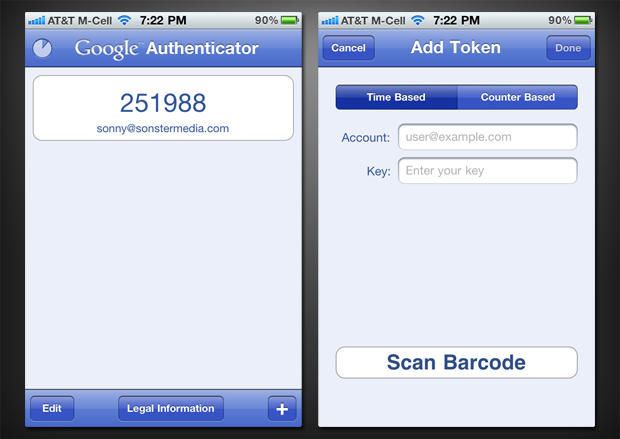
\includegraphics[scale=0.5]{imgHOTP/GoogleAuthenticator_2.jpg}
\end{frame}

  
  OATH Toolkit
  \begin{itemize}
    \item Initiative for Open Authentication (OATH) RAJOUTER DEF ICI OATH Toolkit permet une cr\'{e}ation plus facile des mots de passe uniques des syst\'{e}mes d'authentifications. Il contient 
    une librairie part\'{e}e et un outil de lignes de commandes, et un module PAM.
  \end{itemize}
  
  LinOTP
  \begin{itemize}
    \item LinOTP est une solution bas\'ee Linux pour manager des sys\`{e}tes d'authentifications en deux \'{e}tapes avec un mot de passe unique.
    Il est impl\'{e}ment\'{e} comme un service web bas\'{e} sur le framework python. C'est le seul serveur d'authentification open-source certifi\'{e} par OATH.
  \end{itemize}
  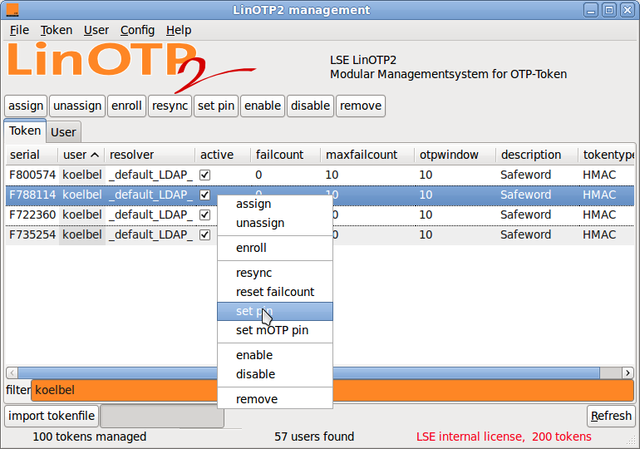
\includegraphics[scale=0.5]{imgHOTP/linOTP.png}
  
  \subsection{Cas d'utilisation envisag\'es}
  Pas trouv\'e
  
\section{Conclusion}
La conclusion
  \subsection{Utilisation dans le cadre du projet}
  Reprendre les \'el\'ements de l'analyse telles que le performances du syt\`eme le niveau de s\'ecurit\'e et autre afin de d\'efinir si, et dans quels contextes, le syst\`eme devrait
  \^etre utlis\'e dans le cadre du projet.
  
  \subsection{Perenit\'e du syst\`eme}
  A voir, pas forc\'ement utile. Se r\'ef\'erer aux r\'esultats de la r\'eunion du 19 novembre.
    

\end{document}

